Come le particelle cariche pesanti, anche gli elettroni e i positroni subiscono una perdita di energia quando attraversano la materia; tuttavia, il fatto che la loro massa sia molto più piccola (basti pensare che la massa di un elettrone è $511 keV$ mentre quella del protone è di circa 1 GeV), fa sì che alcune interazioni non siano più trascurabili. In conseguenza a ciò gli elettroni all'interno della materia seguono percorsi molto più irregolari di quelli delle particelle pesanti, quindi il percorso non può più essere considerato pressoché rettilineo, bensì l'elettrone può cambiare direzione ad ogni interazione importante.

\section{Interazione degli elettroni con la materia}

Cerchiamo allora di capire quali sono i meccanismi mediante i quali gli elettroni perdono energia nella materia.

Mentre per le particelle cariche pesanti il contributo principale è dovuto alle interazioni con gli elettroni atomici e gli altri termini si possono trascurare, per gli elettroni intervengono diversi meccanismi non sempre trascurabili, pertanto la perdita di energia degli elettroni in un mezzo è complessa da calcolare (di solito si stima con programmi/codici, ad esempio GEANT).

I meccanismi attraverso cui gli elettroni perdono energia sono:

\begin{itemize}
    \item Collisioni con elettroni atomici;
    \item Radiazione di frenamento (\textit{bremsstrahlung}): una radiazione elettromagnetica della regione dei raggi X che viene emessa a seguito di un'accelerazione della particella nel campo elettrico nucleare.
\end{itemize}

Quando dobbiamo tenere in considerazione questo ulteriore termine?

Per particelle incidenti aventi basse energie prevale il processo collisionale, similmente alle particelle cariche pesanti, mentre ad alte energie invece prevale il processo radiativo, cioè di bremsstrahlung (viene detto radiativo perché viene emessa radiazione), quindi l'energia viene persa attraverso l'emissione di fotoni $X$.

Osserviamo il seguente grafico: in esso è riportata la perdita di energia specifica in funzione dell'energia della particella, e in particolare troviamo gli andamenti di ciascun termine singolarmente: in blu è riportato l'andamento della perdita di energia per processo collisionale (da notare che ci sono due curve: una per gli elettroni e una per i positroni, che si differenziano leggermente a bassa energia ma poi si unificano), il quale diminuisce rapidamente con l'energia stessa; in rosso è riportato l'andamento dovuto al processo radiativo, il quale va a crescere con l'energia.

La scala è logaritmica rispetto alle ascisse e lineare rispetto alle ordinate; in particolare su quest'ultime è riportata la perdita di energia specifica divisa per l'energia, la quale è espressa in unità di lunghezza di radiazione, che è una grandezza che esprime una quantità proporzionale alla perdita di energia per un dato processo:

\begin{figure}[H]
    \centering
    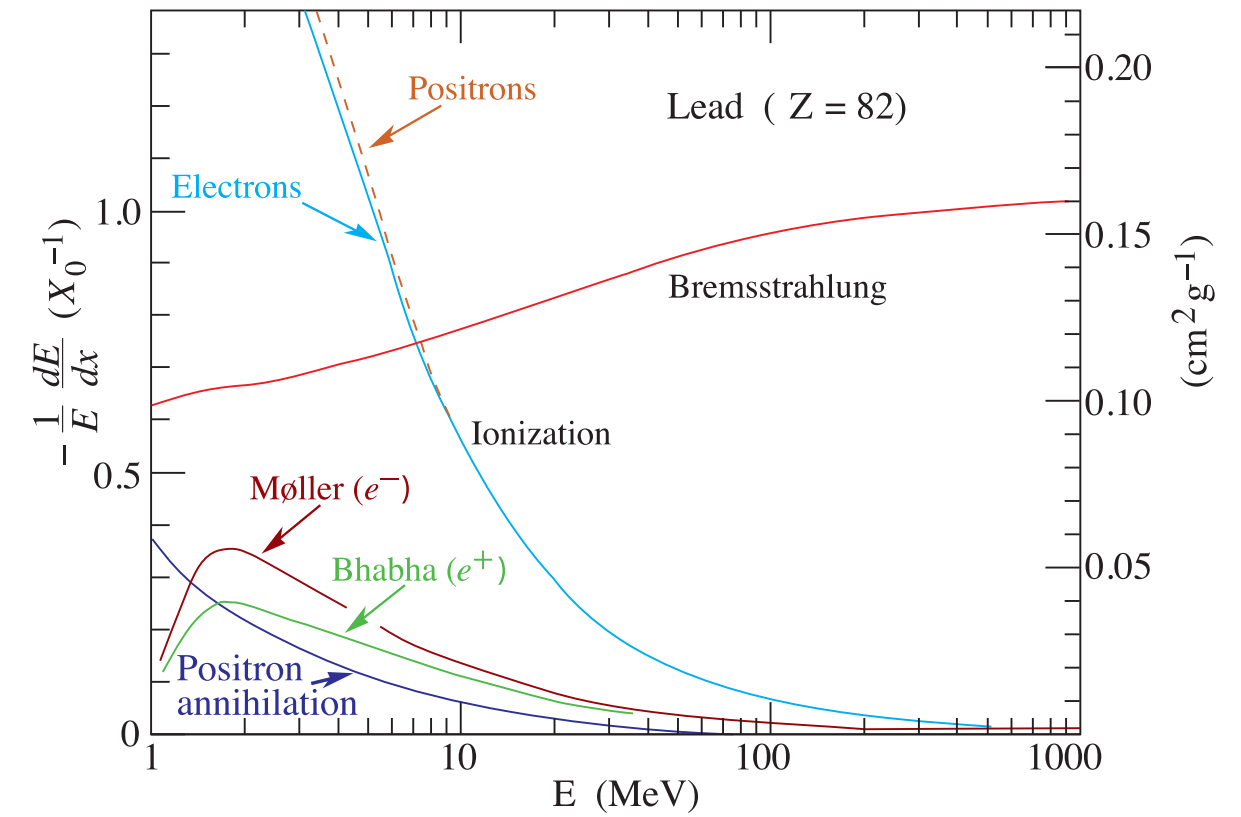
\includegraphics[width=11cm]{immagini/perdita_energia_elettroni.png}
\end{figure}

I due andamenti si incontrano in un punto, in corrispondenza del quale andiamo a valutare la cosiddetta \textbf{energia critica} $E_c$, che è l'energia per la quale i due processi hanno lo stesso contributo, cioè provocano la stessa perdita di energia per unità di percorso:

\begin{equation*}
    \left(\dv{E}{x}\right)_{\rm coll}
    =\left(\dv{E}{x}\right)_{\rm rad}
    \qqtext{per}
    E=E_c
\end{equation*}

Il valore di tale energia dipende dal materiale adoperato (ad esempio nel grafico che è relativo ad elettroni che incidono su piombo si trova a circa 10 MeV).

Da quanto visto deduciamo che se vogliamo calcolare la perdita di energia di un elettrone in un dato spessore di materiale dobbiamo considerare l'energia dell'elettrone, così da capire se è più incisivo il contributo collisionale (basse energie), quello radiativo (alte energie) o se sono confrontabili (intorno al punto critico). Ci potremmo poi chiedere cosa succede quando, per alta energia, vengono emessi fotoni $X$, cioè a cosa danno luogo questi nel materiale, oppure ci potremmo chiedere se a bassa energia intervengono altri fenomeni. Tutto ciò rende il calcolo della perdita di energia difficile da calcolare.

\vspace{0.2cm}Andiamo a vedere i diversi contributi. Si può innanzitutto dire che la perdita di energia specifica per unità di percorso è data dalla somma del contributo collisionale più quello radiativo:

\begin{equation*}
    \left(\dv{E}{x}\right)_{\rm tot}
    =\left(\dv{E}{x}\right)_{\rm coll} + \left(\dv{E}{x}\right)_{\rm rad}
\end{equation*}

\subsection{Contributo collisionale}

Il contributo di collisione è dato da

\begin{equation*}
    \eval{-\dv{E}{x}}_{\rm coll}
    =2 \pi N_a r_e^2 m_e c^2 \rho \frac{Z}{A} \frac{1}{\beta^2} \left[\ln{\left(\frac{\tau^2 (\tau + 2)}{2(I^2/m_e c^2)} + F(\tau) - \delta - 2 \frac{C}{Z}\right)}\right]
\end{equation*}

\E simile alla formula di Bethe-Bloch, ma ci sono alcune differenze. Esse sono dovute al fatto che gli elettroni non percorrono un percorso rettilineo, bensì molto irregolare; inoltre le particelle che incidono sono uguali a quelle con cui vanno a collidere ovvero gli elettroni atomici, per cui c'è una sorta di indistinguibilità tra questi e gli elettroni proiettili.

Compare il termine $\tau$, che rappresenta l'energia incidente in unità della massa dell'elettrone, dato da

\begin{equation*}
    \tau=\frac{E_{k_e}}{m_e c^2}=\gamma - 1
\end{equation*}

Inoltre il figura il termine $F(\tau)$, che vale

\begin{eqnarray*}
    F(\tau)=1 - \beta^2 + \frac{\tau^2/8 - (2\tau + 1)\ln{2}}{(\tau + 1)^2} & \text{per } e^-
    \\
    F(\tau)=2\ln{2} - \frac{\beta^2}{12} \qty[ 23 + \frac{14}{(\tau + 2)} + \frac{10}{(\tau + 2)^2} + \frac{4}{(\tau + 2)^3} ] & \text{per } e^+
\end{eqnarray*}

\subsection{Contributo radiativo}

Prima di affrontare il contributo dovuto alla radiazione, cerchiamo di capire perché non abbiamo preso in considerazione tale termine nel caso di particelle cariche pesanti. Infatti l'emissione di radiazione per bremsstrahlung riguarda un'interazione elettrica tra oggetti carichi, che sono il nucleo e la particella incidente, per cui teoricamente dovremmo considerarla anche nel caso di particelle cariche pesanti. Tuttavia, se guardiamo in dettaglio la forma della sezione d'urto per tale processo si trova la seguente proporzionalità:

\begin{equation*}
    \dv{\sigma}{E} \propto \frac{Z^2}{m_i^2} \frac{\ln{E}}{E}
\end{equation*}

dove $Z$ è relativo al materiale. Tale proporzionalità è dovuta al fatto che, trattandosi di un processo di interazione tra la particella è il nucleo, se quest'ultimo ha una nuvola di elettroni questa darà un effetto di schermaggio.

Ciò che è più importante però è la dipendenza dall'inverno del quadrato della massa della particella incidente, che è il motivo per cui non consideriamo tale contributo per le particelle cariche pesanti: la sezione d'urto diminuisce all'aumentare della massa.

Per quantificare facciamo un confronto tra la sezione d'urto dovuta a tale processo per elettroni e muoni, i quali hanno una massa di 207 volte quella degli elettroni. A parità di energia e se consideriamo lo stesso materiale tale rapporto si riduce al rapporto tra i quadrati delle masse, che risulta valere

\begin{equation*}
    \qty(\frac{m_{e}}{m_{\mu}})^2
    =\frac{1}{37000}
\end{equation*}

Tale esempio ci mostra perché tale contributo sia normalmente trascurabile\footnote{Ad energie molto elevate, ad esempio nel caso di acceleratori di particelle, va considerato.}.

La perdita di energia specifica dovuta alla radiazione di frenamento è data da

\begin{equation*}
    \eval{-\dv{E}{x}}_{\rm rad}
    =4 Z^2 r^2 \alpha \left[ \ln{\qty(183Z^{-\frac{1}{3}})} + \frac{1}{18} - f(Z) \right]NE
\end{equation*}

il fatto che ci sia il termine $Z^2$ ci dice che la perdita di energia dipende dal materiale attraversato.

\subsection{Energia critica}
Concentriamoci ora sull'energia critica.

\begin{minipage}{0.495\textwidth}
    \begin{figure}[H]
        \centering
        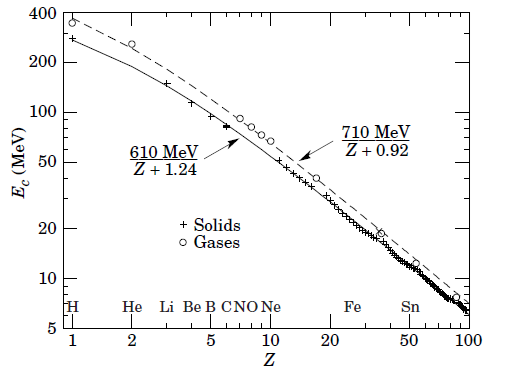
\includegraphics[width=8cm]{immagini/energia_critica.png}
    \end{figure}
\end{minipage}
\begin{minipage}{0.5\textwidth}
    \vspace{0.3cm}Siccome la sezione d'urto è complessa, non è facile avere una formula teorica per calcolare l'energia critica, per cui si fanno diverse parametrizzazioni.
    
    Nel grafico è riportato il valore di energia critica espresso in MeV e in funzione di $Z$, quindi man mano passiamo da elementi più leggeri a elementi più pesanti. Ci sono due parametrizzazioni: una per i solidi e una per il gas.
\end{minipage}

\vspace{0.3cm}In base al valore di energia critica possiamo capire se bisogna tenere conto del contributo radiativo oppure no. Ad esempio, in laboratorio, per studiare la perdita di energia degli elettroni attraverso spessori di vari materiali come ad esempio l'alluminio, adoperiamo delle sorgenti $\beta$ di stronzio e ittrio poco energetiche, che hanno un endpoint dello spettro intorno a $2.3$ MeV; dal grafico però si evince che l'energia critica per l'alluminio ($Z=13$) è di circa 40 MeV, per cui la perdita di energia è imputabile totalmente al processo collisionale.

Vediamo altri esempi di curve di perdita di energia sia complessiva che dovuta singolarmente ai due processi:

\begin{esempio}
    In figura è riportata in nero la perdita di energia complessiva degli elettroni per due materiali diversi (alluminio a sinistra e ferro a destra).
    
    Notiamo come gli elettroni inizialmente, per basse energie, hanno una perdita di energia abbastanza elevata che va diminuendo fino ad un minimo, ed il motivo di tale andamento è che in tale regione interviene principalmente il meccanismo di perdita di energia collisionale, che ha appunto un andamento discendente. Dopo il minimo si risale soprattutto a causa del termine radiativo, ed infatti fino a energie dell'ordine del MeV la curva complessiva e quella del contributo collisionale coincidono. Il contributo radiativo invece assume inizialmente dei valori molto bassi per poi diventare preponderante al di sopra della decina di MeV.
    \begin{figure}[H]
        \centering
        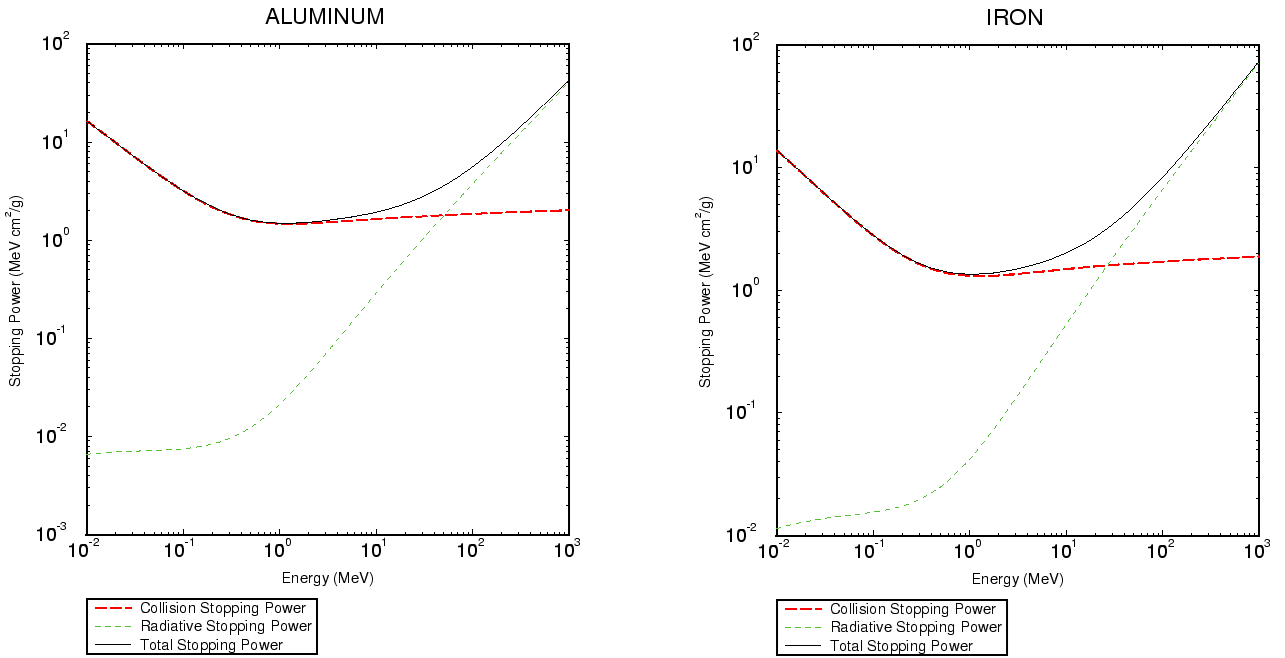
\includegraphics[width=\textwidth]{immagini/esempi_energy_loss_elettroni.png}
    \end{figure}
    Dai due grafici evinciamo come il punto critico cambi in base al tipo di materiale.
\end{esempio}

\begin{esempio}
    In figura è riportata la perdita di energia di elettroni nel caso del cemento.
    \begin{figure}[H]
        \centering
        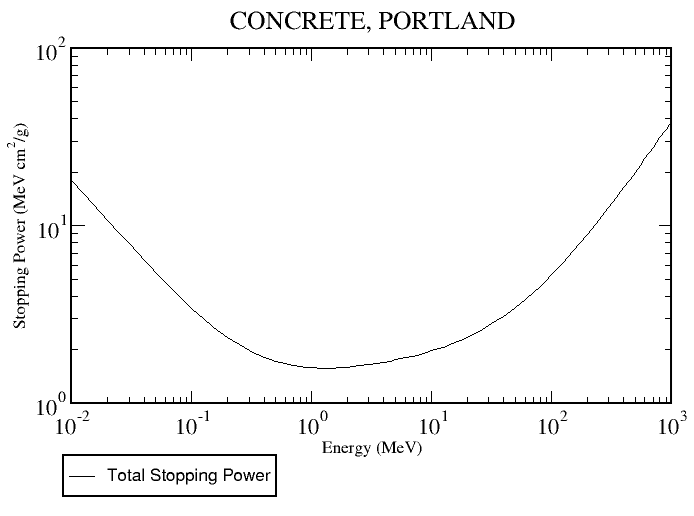
\includegraphics[width=0.6\textwidth]{immagini/energy_loss_elettroni_cemento.png}
    \end{figure}
    Se ad esempio volessimo studiare l'effetto di schermaggio che produce un solaio di un qualsiasi edificio relativo agli elettroni della radiazione cosmica, un grafico di questo tipo permette di stimare qual è il minimo valore di energia che deve avere un elettrone cosmico per poter attraversare un determinato spessore di cemento.
\end{esempio}

\newpage

\subsection{Riepilogo}

Riassumendo:

\begin{center}
    \begin{tabular}{p{6.7cm}p{0.8cm}p{6.7cm}}
        \hspace{2cm}Processo collisionale \hspace{2cm} & & \hspace{2cm}Bremsstrahlung\\[0.5cm]
        $\displaystyle \dv{E}{x}$ varia linearmente con $Z$;\footnotemark & & $\displaystyle \dv{E}{x}$ varia quadraticamente con $Z$;\\[0.5cm]
        Domina a energie minori di quella & & Domina a energie maggiori di quella\\
        critica; & & critica;\\[0.2cm]
        L'energia è ceduta al materiale as- & & L'energia è ceduta ai fotoni;\\
        sorbente (agli elettroni atomici); & &\\[0.2cm]
        Avvengono molte collisioni, quindi & & Pochi fotoni emessi.\\
        la perdita di energia è graduale. & &
    \end{tabular}
\end{center}

\footnotetext{Tale dipendenza ci dice che la scelta del materiale è più incisiva sul contributo radiativo.}

\section{Range degli elettroni}

A causa della maggiore suscettibilità dell'elettrone allo scattering multiplo da parte dei nuclei, il range degli elettroni è generalmente molto diverso dalla lunghezza del percorso calcolata mediante integrazione della formula del $\dv*{E}{x}$:

\begin{equation*}
    \text{range} \neq \int \qty( \dv{E}{x} )^{-1} \dd{E}
\end{equation*}

Spesso si riscontrano differenze che vanno dal 20\% al 400\% a seconda dell'energia e del materiale. Inoltre, la perdita di energia da parte degli elettroni oscilla molto di più che per le particelle pesanti. Ciò è dovuto al trasferimento di energia molto maggiore per collisione consentito per gli elettroni e all'emissione di bremsstrahlung. In entrambi i casi è possibile che poche singole collisioni (o fotoni) assorbano la maggior parte dell'energia dell'elettrone. Ciò ovviamente si manifesta in effetti ancora maggiori di straggling e quindi il concetto di range diventa ancora meno definito di quanto non lo fosse per le particelle cariche pesanti. %Infatti, anche se inviamo due elettroni con la stessa energia verso lo stesso materiale, ognuno seguirà un percorso molto diverso dagli altri, fatto che produce valori di range diversi.

\begin{figure}[H]
    \centering
    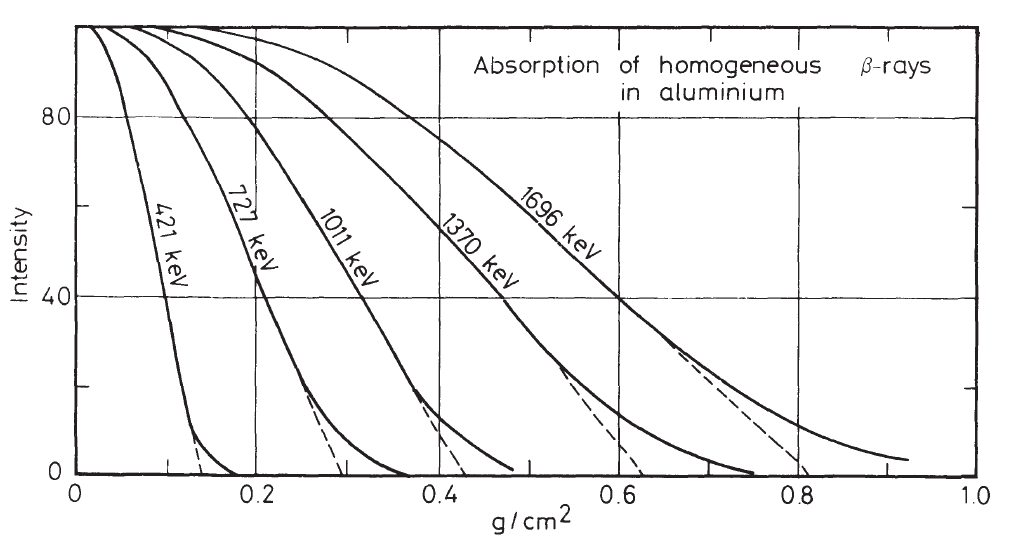
\includegraphics[width=0.8\textwidth]{immagini/range_elettroni.png}
\end{figure}

In tale grafico è rappresentato il coefficiente di trasmissione\footnote{Se guardiamo attentamente il grafico notiamo che in realtà in ordinate è riportata l'intensità del fascio, ciò però non è rilevante in quanto per ottenere il coefficiente di trasmissione basta dividere per $I_0$, che è un valore costante.} in funzione del percorso effettuato in un materiale espresso in unità di densità superficiale\footnote{Il fatto che esprimiamo lo spessore in termini di densità superficiale rimuove la dipendenza dalla densità del materiale. In conseguenza a ciò, cambiando materiale il grafico cambierà di poco, mentre se esprimessimo lo spessore in unità di lunghezza si osserverebbero notevoli variazioni.}. Le varie curve sono ottenute per fasci di elettroni mono-energetici ad energie diverse.

Notiamo come gli elettroni meno energetici percorrono meno spazio nella materia e la curva scende rapidamente ed è molto smussata, per cui non si può identificare un gradino come per le particelle cariche pesanti. Tuttavia anche qui possiamo ricavare il range o considerando il range medio (ovvero la distanza percorsa da almeno metà delle particelle incidenti) o il range estrapolato (l'intersezione della tangente alla curva nel punto medio con l'asse delle ascisse, in figura rappresentata dalla linea tratteggiata). All'aumentare dell'energia degli elettroni la curva si sposta verso valori più elevati, l'andamento smussato persiste ed il range diventa ancora meno definito.

In realtà in natura i raggi $\beta$ non sono monocromatici, cioè non vengono emessi a precisi valori di energia, in quanto lo spettro del decadimento $\beta$ è continuo. \E quindi chiaro che queste curve sono state ottenute selezionando mediante campi magnetici elettroni con date energie. Infatti gli elettroni vengono deviati con un raggio di curvatura che dipende dall'energia, per cui posizionando il rivelatore ad un certo angolo di deviazione andiamo a selezionare elettroni di una certa energia. L'energia con cui possiamo sceglierli diventa sempre più precisa al restringersi dell'angolo solido, per cui spesso si usano dei collimatori, strumenti che vanno a selezionare una porzione del fascio (come un ostacolo con un foro, per cui misuriamo solo quello che passa dal foro).

Nella realtà quindi non troveremo elettroni monocromatici (mono-energetici), bensì ad energie diverse, per cui sperimentalmente, effettuando un esperimento di trasmissione, avremo a disposizione elettroni con energie molto piccole, anche prossime allo zero, e altri con energie di alcuni MeV, con una proporzione che dipende dallo spettro di emissione. Nel caso di stronzio-90 e ittrio-90 prevalgono le energie più basse, per cui ci aspettiamo una curva tendenzialmente a sinistra. Ne segue che quando effettuiamo un esperimento di trasmissione si deve fare una convoluzione, nel senso che ci saranno più curve, ciascuna per una certa energia, pesate rispetto al numero di particelle aventi tale energia.

\section{Assorbimento degli elettroni}
Poiché gli elettroni assumono valori continui di energia, quello che poi andiamo a misurare in laboratorio è un andamento più simile ad un esponenziale decrescente. I fattori che determinano tale andamento sono lo spettro continuo dei $\beta$ e lo straggling (il quale rende la curva smussata).

Una rappresentazione semi-empirica dell'assorbimento degli elettroni si ha tramite la legge

\begin{equation*}
    I=I_0 e^{-\mu x}
\end{equation*}

da cui segue immediatamente che il coefficiente di trasmissione avrà il seguente andamento:

\begin{equation*}
    T=\frac{I}{I_0}=e^{-\mu x}
\end{equation*}

dove $x$ è lo spessore attraversato e $\mu$ è il \textit{coefficiente di assorbimento degli elettroni}, un parametro che dipende dal tipo di materiale e che rappresenta la pendenza della curva in figura, che ha la forma di un relazione lineare perché le ordinate sono riportare in scala logaritmica.

\begin{minipage}{0.495\textwidth}
    \begin{figure}[H]
        \centering
        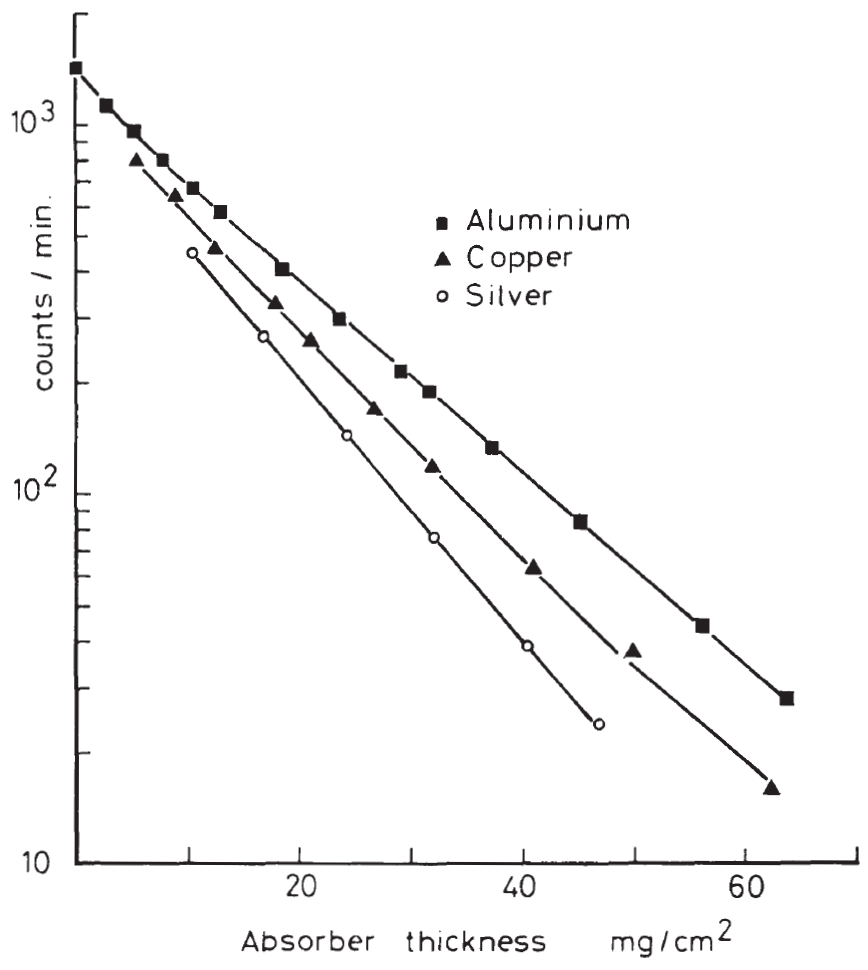
\includegraphics[width=7cm]{immagini/assorbimento_elettroni.png}
    \end{figure}
\end{minipage}
\begin{minipage}{0.5\textwidth}
    Nel grafico è riportato il numero di elettroni che attraversano un determinato spessore di materiale (espresso in unità di densità superficiale) per diversi materiali.
    
    $\mu$ rappresenta quindi la capacità di assorbimento di un dato materiale: tanto più è grande, tanto più il materiale riesce ad assorbire gli elettroni. Si esprime in $\rm cm^{-1}$ o in $\rm cm^2/g$ (perché deve dare un numero puro).

    In particolare il termine $1/\mu$ rappresenta lo spessore necessario a ridurre il flusso iniziale di un fattore $1/e$:

    \begin{equation*}
        x=\frac{1}{\mu}
        \implies
        I=I_0 e^{-\frac{\mu}{\mu}}
        =\frac{I_0}{e}
    \end{equation*}
\end{minipage}

\vspace{0.2cm}Lo scopo dell'esperienza è quindi trovare i vari punti e realizzare un best-fit lineare per valutare $\mu$. I vari punti corrispondono a diversi spessori in corrispondenza dei quali calcoliamo $I/I_0$. Per linearizzare la formula si fa un passaggio ai logaritmi:

\begin{equation*}
    \log{\qty(\frac{I}{I_0})}
    =\log{\qty(e^{-\mu x})}
    =-\mu x
\end{equation*}

\section{Backscattering}

\begin{minipage}{0.245\textwidth}
    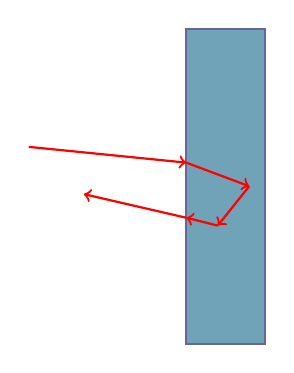
\begin{tikzpicture}
        \draw[blue!20!gray,thick,fill=gray!60!cyan] (0,0) rectangle (1cm,4cm);
        \draw[thick,red,->] (-2,2.5) -- (0,2.3);
        \draw[thick,red,->] (0,2.3) -- (0.8,2);
        \draw[thick,red,->] (0.8,2) -- (0.4,1.5);
        \draw[thick,red,->] (0.4,1.5) -- (0,1.6);
        \draw[thick,red,->] (0,1.6) -- (-1.3,1.9);
      \end{tikzpicture}
\end{minipage}
\begin{minipage}{0.75\textwidth}
    Nella materia gli elettroni, durante il loro percorso, variano di molto la loro direzione. Tale effetto è tanto più evidente quanto più bassa è l'energia dell'elettrone; nel caso di elettroni a bassissima energia si può anche verificare il fenomeno del \textit{backscattering}, cioè scattering all'indietro: l'elettrone, a seguito delle diverse collisioni, ritorna indietro. Sperimentalmente esso rappresenta un rischio perché potremmo perdere segnale in quanto tali elettroni non vengono rivelati né depositano tutta la loro energia.
\end{minipage}

\vspace{0.4cm}Il motivo per cui subiscono tale processo è che gli elettroni sono particelle di massa molto piccola, il che le rende particolarmente suscettibili a deflessioni di un grande angolo a seguito dello scattering coi nuclei; il perché tale fenomeno sia più evidente a basse energie è una conseguenza dei calcoli (aumenta la probabilità di avere scattering ad angoli più grandi), ma classicamente ce lo possiamo spiegare immaginando di trovarci in una stanza in cui sono presenti tante persone e di voler passare da una parte all'altra: se passiamo lentamente (quindi bassa energia cinetica) collidiamo e abbiamo difficoltà a muoverci in maniera rettilinea, mentre se passiamo correndo (quindi alta energia cinetica) scansiamo alcune persone e riusciamo a muoverci in linea dritta.

\begin{approfondimento}[Perché il fenomeno del backscattering per gli elettroni è più evidente a basse energie?]
    \footnotesize Questa risposta me l'ha data chatgpt, ma mi sembra interessante riportarla.

    \vspace{0.2cm}Il fenomeno del backscattering per gli elettroni è più evidente a basse energie principalmente a causa delle interazioni tra gli elettroni e il materiale target, che dipendono fortemente dall'energia degli elettroni incidenti. Vediamo alcuni punti chiave che spiegano questo comportamento:

    \begin{enumerate}[leftmargin=0.6cm]
        \item Interazioni elastiche e inelastiche:
        \begin{itemize}[leftmargin=0pt]
            \item Interazioni elastiche: A basse energie, le interazioni elastiche tra gli elettroni incidenti e gli atomi del materiale sono più frequenti. In queste interazioni, gli elettroni possono essere deviati indietro (backscattered) con una probabilità maggiore.
            \item Interazioni inelastiche: Quando l'energia degli elettroni incidenti è alta, le interazioni inelastiche, in cui gli elettroni perdono energia attraverso l'eccitazione o la ionizzazione degli atomi del materiale, diventano più dominanti. Questo riduce la probabilità che gli elettroni vengano retro-diffusi, poiché tendono a penetrare più profondamente nel materiale e perdere energia piuttosto che essere riflessi indietro.
        \end{itemize}
        \item Penetrazione nel materiale:
        \begin{itemize}[leftmargin=0pt]
            \item A basse energie, gli elettroni penetrano meno nel materiale a causa della loro minore energia cinetica. Questo significa che hanno maggiori probabilità di interagire con gli atomi superficiali del materiale e di essere riflessi indietro.
            \item A energie più alte, gli elettroni possono penetrare più in profondità nel materiale, riducendo la probabilità di backscattering poiché le loro traiettorie sono meno influenzate dalle interazioni con gli atomi superficiali.
        \end{itemize}
        \item Scattering angolare:
        \begin{itemize}[leftmargin=0pt]
            \item A basse energie, l'angolo di scattering degli elettroni a seguito di interazioni elastiche è più grande. Questo significa che gli elettroni sono più facilmente deviati verso angoli maggiori, inclusi angoli prossimi a 180 gradi (backscattering).
            \item A energie più alte, l'angolo di scattering tende a essere più piccolo, e quindi gli elettroni sono meno probabilmente retro-diffusi.
        \end{itemize}
        \item Effetto del potenziale nucleare:
        \begin{itemize}[leftmargin=0pt]
            \item Gli elettroni a basse energie sono più influenzati dal potenziale coulombiano del nucleo degli atomi del materiale. Questo può causare una maggiore deflessione indietro degli elettroni incidenti.
            \item A energie più alte, gli elettroni hanno meno probabilità di essere significativamente deviati dal potenziale nucleare a causa della loro maggiore velocità e momento.
        \end{itemize}
    \end{enumerate}
    In sintesi, il backscattering degli elettroni è più evidente a basse energie perché le interazioni elastiche sono più frequenti e dominanti, gli elettroni penetrano meno nel materiale e sono più facilmente deviati verso angoli maggiori.
\end{approfondimento}

Oltre che dall'energia, il processo di backscattering dipende anche dal numero atomico $Z$ del materiale.

Il backscattering si quantifica tramite il \textit{coefficiente di backscattering}, che rappresenta il rapporto tra il numero di elettroni che vengono backscatterati rispetto al numero di elettroni incidenti. Talvolta viene chiamato anche \textit{albedo}\footnote{Termine preso in prestito dall'astrofisica e che rappresenta la luce riflessa da un corpo opaco, in quanto in questo caso abbiamo degli elettroni che incidono su una superficie e in parte vengono riflessi all'indietro.}. Per come è definito segue che esso può valere al massimo 1 (o 100\%).

\begin{figure}[H]
    \centering
    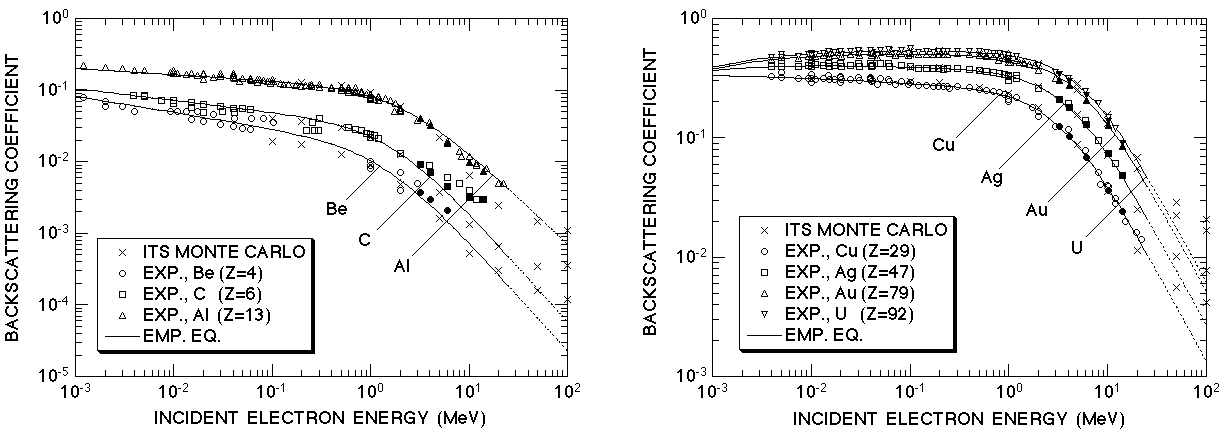
\includegraphics[width=\textwidth]{immagini/esempi_backscattering.png}
\end{figure}

I grafici riportano i valori del coefficiente di backscattering in funzione dell'energia dell'elettrone. Come detto prima è elevato ad energie basse e diminuisce all'aumentare dell'energia in modo drastico (da notare che le scale adoperate sono logaritmiche), per cui ad alte energie è un effetto trascurabile. Il fatto che ci siano curve diverse per materiali diversi ci dice che c'è una dipendenza anche dal tipo di materiale. In particolare il backscattering è meno evidente per materiali più leggeri, per cui il coefficiente è più piccolo. Nei materiali più pesanti (grafico a destra) invece questo effetto prevale anche per energie dell'ordine del MeV e non si può trascurare.

\comment{
\textbf{continua a 1:05:10 circa}

\section{Scattering multiplo}

Il percorso seguito da una particella può essere più o meno frastagliato, cioè con più o meno deviazioni. Studiamo ora nel dettaglio i motivi per cui si devia dal percorso rettilineo.

Il maggiore contributo al processo di deflessione e dato dai processi coulombiani (in misura minore anche dalla interazione nucleare). Ciò che si fa è distinguere tre casi principali:

\begin{enumerate}
    \item Se lo spessore adoperato è particolarmente sottile siamo nel caso in cui con buona probabilità si verifica un singolo scattering all'interno dello spessore. Esso può essere affrontato con lo scattering Rutherford, in cui la sezione d'urto è funzione dell'angolo di scattering;
    \item Se lo spessore adoperato è considerevole il numero di scattering è elevato (\textit{multiple scattering}), come avviene nella maggior parte dei casi reali. La particella quindi, nell'attraversare il materiale, subisce delle deflessioni dovute a diverse collisioni. Essendo il numero di queste elevato, tale processo si studia da un punt di vista statistico;
    \item Il caso intermedio è quello del \textit{plural scattering}, ed è il caso in cui il numero di collisioni è minore di 20. Poiché tale numero non è levato, il fenomeno non può essere studiato dal punto di vista statistico ed è difficile farne una trattazione.
\end{enumerate}

Concentriamoci sul secondo caso. La teoria statistica che ci permette di studiare l'angolo di fuoriuscita di una particella dopo aver attraversato un dato spessore è la teoria di Moliere.

Immaginiamo di avere un percorso all'interno di un materiale di lunghezza $x$:

\vspace{-0.2cm}

\hspace{-0.2cm}\begin{minipage}{0.495\textwidth}
    \begin{figure}[H]
        \centering
        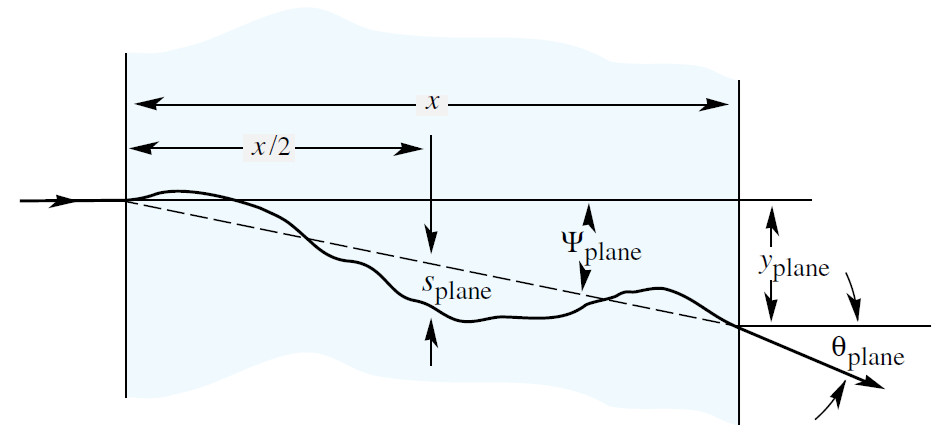
\includegraphics[width=8cm]{immagini/scattering_multiplo_1.png}
    \end{figure}
\end{minipage}
\hspace{0.2cm}\begin{minipage}{0.5\textwidth}
    \vspace{0.6cm}Una volta che la particella entra nello spessore subisce una serie di scattering multipli che fanno deviare continuamente la particella del suo percorso rettilineo. Se quindi andiamo a vedere la fuoriuscita dal materiale, la particella potrebbe essere spostata rispetto all'altezza in ingresso e potrebbe aver cambiato direzione incidente, formando un angolo $\vartheta$ rispetto a quello di partenza.
\end{minipage}

\vspace{0.2cm}L'effetto dello scattering multiplo può essere studiato attraverso questa deviazione, cioè possiamo fare delle considerazioni statistiche sull'angolo di uscita. In particolare la distribuzione dell'angolo di scattering è di tipo gaussiano per piccoli angoli, mentre per grandi angoli ha una coda a valori più alti di quelli previsti da una gaussiana. Ciò vuol dire che in media, se inviamo delle particelle e studiamo l'angolo di deflessione in uscita, ci aspettiamo che nella maggior parte dei casi si mantenga la direzione di partenza e via via diventa sempre più improbabile che l'angolo di deflessione sia elevato.

\E da notare che la figura di sopra affronta il problema nel caso planare ma in realtà si tratta di un problema tridimensionale, cioè dovremmo studiare l'angolo tra due direzioni nello spazio; è tuttavia equivalente considerare la proiezione su un piano.

Una prima conclusione è quindi che la deviazione media nel piano è zero (la media dei vari angoli di uscita). Maggiormente però ci interessa la larghezza della distribuzione, cioè di quanto varia, da evento a evento, l'angolo di deviazione, ossia la dispersione di questi angoli. Se indichiamo con $\vartheta_0$ la larghezza della distribuzione, essa può essere definita andando a valutare lo scarto quadratico medio dei vari $\vartheta_{\rm plane}$ (rms\footnote{chatgpt dice che sta per "radial mean square", ma sec me bisognerebbe chiedere}). La relazione tra rms del piano e quello dello spazio è

$$\vartheta_0=\vartheta_{\rm plane}^{\rm rms}
=\frac{1}{\sqrt{2}} \vartheta_{\rm space}^{\rm rms}$$

Maggiore è il valore di rms, più si evidenziano effetti di scattering multiplo. L'rms dipenderà da:

\begin{itemize}
    \item Il tipo di particelle incidente;
    \item L'energia o l'impulso della particella incidente;
    \item Le proprietà del materiale.
\end{itemize}

Dalla teoria di Moliere si ricava che, assumendo una distribuzione Gaussiana per l'angolo di scattering nel piano, la sua larghezza è data da:

$$\vartheta_0=\frac{13.6 \; \text{MeV}}{\beta c p} z \sqrt{x/X_0} \big[ 1 + 0.038 \ln(x/X_0) \big]$$

dove $p$ è l'impulso particella, $x$ lo spessore del materiale, $z$ il numero atomico della particella e $X_0$ la lunghezza di radiazione del materiale.

\subsection{Lunghezza di radiazione}

\E un parametro caratteristico del materiale. \E legato all'interazione degli elettroni o dei fotoni di alta energia, ma utilizzato in diversi contesti.

Si può definire in due modi:

\begin{itemize}
    \item come la distanza media entro cui un elettrone ad alta energia riduce la sua energia ad $1/e$ del valore iniziale mediante processi di radiazione (bremsstrahlung);
    \item come $7/9$ del libero cammino medio per produzione di coppie da parte di un fotone di alta energia.
\end{itemize}

Dalla prima definizione capiamo che più il materiale assorbe l'energia dell'elettrone, più la lunghezza di radiazione è piccola. Ricordiamo inoltre che i fotoni interagiscono con la materia attraverso tre meccanismi principali: effetto fotoelettrico, effetto Compton e la produzione di coppie elettrone-positrone.

\textbf{continua}

$$L_r=\frac{716.4 \; A}{Z(Z+1)\ln(287/\sqrt{z})}
\quad \rm \qty[g/cm^2]$$

\subsection{Distribuzione angolare di scattering}

\begin{figure}[H]
    \centering
    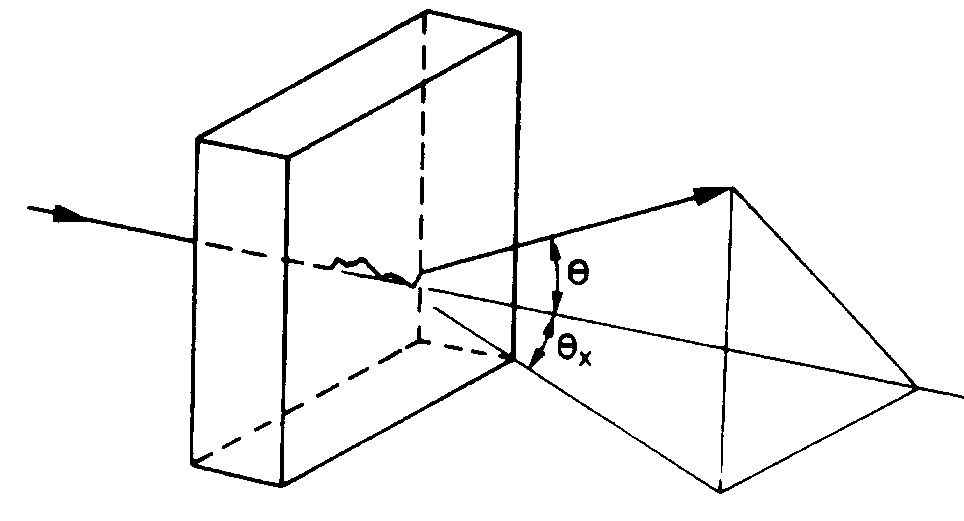
\includegraphics[width=8cm]{immagini/distribuzione_angolare_di_scattering.png}
\end{figure}

$$\frac{1}{2 \pi \vartheta_0^2}e^{\left(-\frac{\vartheta_{\rm space}^2}{2\vartheta_0^2}\right)}d \Omega$$

\subsection{Conseguenze dello scattering multiplo}

\textbf{rileggi}In generale lo scattering multiplo comporta una deviazione rispetto alla direzione di partenza. In alcuni casi è importante dover stimare tale scattering (\textbf{o deviazione boh vai a vedere la lez}), ad esempio nel caso in cui vogliamo tracciare una particella: immaginiamo di avere una collisione tra nuclei o protoni da cui emergono tantissime particelle (è quello che viene negli acceleratori LHC) e vogliamo non solo capire che tipo di particelle vengono emesse, ma anche il percorso. Per fare ciò si usano dei \textit{rivelatori di tracciamento} che vanno a individuare, attraverso dei punti, il percorso che seguono. Essendo fatto di materia, ogni volta che una particella colpisce un rivelatore subisce scattering multiplo, quindi tutto ciò che misurano i rivelatori e successivi risentirà dello scattering multiplo provocato dai rivelatori precedenti. Ne segue che quando ricostruire la traccia di una particella (ad esempio rettilinea), non ci aspetteremo dei punti allineati, bensì dovremo considerare dei margini che tengono conto del fatto che la particella non segue un percorso rettilineo, ma nell'attraversare un materiale ha subito una leggera deviazione (scattering multiplo) per questa ragione, dato che i rivelatori non devono fermare la particella e devono deviare la sua traiettoria il meno possibile, parte dello sviluppo di un rivelatore consiste nel cercare di ridurre il "material budget", cioè la quantità di materia che si introduce attraverso l'inserimento di un rivelatore (nel caso ideale tale budget è nullo).

Un altro caso in cui è importante stimarlo è per misurare la direzione di arrivo dei raggi cosmici, i quali vengono deviati attraversando l'aria.

Va ricordato che questo effetto è importante per particelle di basso impulso e per materiali ad alto $Z$.
}